\documentclass[12pt]{My_preprint}
\title{
    Statistical modeling of the \textit{Flotation} process.  
    }

\author[1,2]{Nicolas Fintzi}
\normalmarginpar

\renewcommand*\contentsname{}
\begin{document}

\maketitle


\begin{abstract}
    Based on the averaged equations for dispersed multiphase flows \citep{jackson2000} we derive a criterion for the minimal height $L$ of a cylindrical flotation column (specifically, dissolved air flotation). 
    We start with a brief summary of the results, then we apply the results to a few examples of flotation columns (``CleanWash'', ``Colonne labo Solaize'') determining their ideal size. 
    The details of the theory are given afterward, from the local-scales equations governing the fluid to the macroscopic 3D equation and finally the 1D model.
    A significant discrepancy with existing literature has been identified during the re-derivation of the collision kernel in viscous uniform flows.
    By incorporating the Faxén force acting on particles immersed in the wake of bubbles, we demonstrate that conventional formulas commonly used in the literature \citep{loewenberg1994flotation} underestimate the collision efficiency by a factor of  $1/4$.   
\end{abstract}
\tableofcontents
\newpage

\section{Summary of the method and main results}
\label{sec:summary}
\begin{figure}[h!]
    \centering
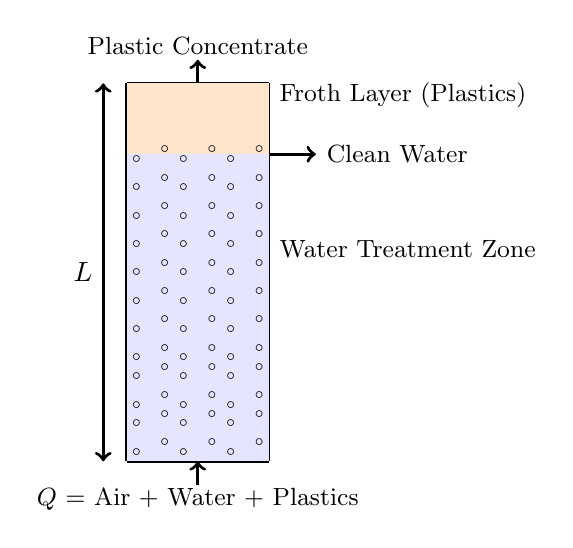
\begin{tikzpicture}[scale=0.6,very thick]

    % Column body
    \draw (0,0) -- (0,8);
    \draw (3,0) -- (3,8);
    \draw (0,8) -- (3,8);
    \draw (0,0) -- (3,0);
    
    % Height label L
    \draw[<->] (-0.5,0) -- (-0.5,8)node[midway, left]{$L$};
    
    % Froth zone (microplastics)
    \fill[orange!20] (0,6.5) rectangle (3,8);
    \node[right] at (3,7.75) {\small Froth Layer (Plastics)};
    
    % Water treatment zone
    \fill[blue!10] (0,0) rectangle (3,6.5);
    \node[right] at (3,4.5) {\small Water Treatment Zone};
    
    % Air+Water+Plastic inlet
    \draw[ ->] (1.5,-0.5) -- (1.5,0);
    \node at (1.5,-0.8) {\small $Q$ = Air + Water + Plastics};
    
    % Clean water outlet (side)
    \draw[ ->] (3,6.5) -- (4,6.5);
    \node[right] at (4,6.5) {\small Clean Water};
    
    % Plastic concentrate outlet (top)
    \draw[ ->] (1.5,8) -- (1.5,8.5);
    \node at (1.5,8.8) {\small Plastic Concentrate};
    
    % Bubbles
    \foreach \y in {1.2, 1.8,0.2, 0.8,2.2, 2.8, 3.4, 4.0, 4.6, 5.2, 5.8, 6.4} {
      \node at (1.2,\y) {\tiny $\circ$};
      \node at (1.8,\y+0.2) {\tiny $\circ$};
      \node at (0.2,\y) {\tiny $\circ$};
      \node at (0.8,\y+0.2) {\tiny $\circ$};
      \node at (2.2,\y) {\tiny $\circ$};
      \node at (2.8,\y+0.2) {\tiny $\circ$};
    }
\end{tikzpicture}
\caption{Sketch of a typical the flotation column with high $L$. The input flow rate $Q$ is usually imposed by the upstream processes.  The goal of this study is then to predict the output of ``Plastic concentrate''  and the high $L$ in terms of the input flow rate $Q$. }
\end{figure}


\subsection{Definitions}
Let us first introduce a series of dimensionless numbers: 
\begin{align*}
    \xi = d_b / d,
    && L^* = L / d,
    && \zeta = \rho_b / \rho_f,
    && \lambda = \mu_b / \mu_f,\\
    \phi_b = V_b/V_{tot},
    && \phi_p = V_p/V_{tot}.
    && \phi_p^a = V_p^a/V_{tot}.
    && X\% = \phi_p^a /\phi_p\\
    &&
    Re = |\textbf{u} - \textbf{u}_b|\rho_f d /\mu_f ,
    && Ga = d^3 g\rho_f^2 (1-\zeta)/\mu_f^2. 
\end{align*}
$d$ and $d_p$ are the diameter of the spherical bubbles and particles, respectively.
$L$ is the height of the flotation column. 
$\mu_k$  and $\rho_k$ are the viscosity and density of the phase $k$. 
$V_k$ is the total volume of phase $k$. 
$V^a_k$ corresponds to the volume of attached particles (number of attached particles times the volume of a single particle). 
``$k$'' represents either the bubbles phase ($k=b$), the water phase ($k=f$), or the particles phase ($k=p$).
$g = 9.81$ m.s$^{-2}$ represents the gravity acceleration. 
$\textbf{u} = \phi_p \textbf{u}_p + \phi_b \textbf{u}_b + \textbf{u}_f(1-\phi_b+\phi_p)$ represents the velocity of the mixture, $\textbf{u}_k$ being the mean velocity of phase $k$.

With these definitions $Ga$ is the \textit{Galileo} number, comparing viscous to buoyancy forces, and $Re$ is the bubbles Reynolds number, comparing viscous drag force and inertial forces acting on the bubbles.
$\phi_k$ the volume fractions of each phase. 
And $X\% $ the percentage of attached particles in the column. 

The objective of this study is to determine $L^*$ for a given $X\%$.
In the ideal scenario we would like to clean $100\%$ of waste in the water, this corresponds to $X\%=1$, however we will see that due to the asymptotic behavior of the function $L^* (X\%)$ one may only be able to reach $X\% \approx 0.9$ in order to keep a height $L$ of the order of the meter. 

\subsection{Governing equations}

In a first modeling attempt we need to state a consequent number of assumptions. 
These will be relaxed in future studies however for instance we consider that:
\begin{enumerate}
    \item The flow (meaning the bulk and bubbles and particles velocity) is established along the columns and at steady-state.
    \item Plug flow: $\textbf{u}$, $\textbf{u}_b$ and $\textbf{u}_p$ are constant across the section. That means that we neglect the effects of the sides of the column on the flow.
    \item The two previous hypothesis also apply to the concentration fields $\phi_k$. 
    However, $\phi^a_p$ varies along the column height as bubbles catch free particles in the flow while rising. 
    \item $\phi_p\ll \phi_b<0.25$ and $Ga<100$ : This is not too restrictive as in the real processes this criterion are often respected. 
    \item $\xi \ll 1$: The collision efficiency is computed such that we neglect the $O(\xi^3)$ (see~\ref{sec:efficiency}) term hence $\xi$ must be reasonably low. 
    \item $Re_p\ll 1$: Due to their small size, the particles are considered inertialess, such that they be assimilated to tracers in the ambient fluid. 
\end{enumerate}

With these assumptions into hand the modeling process goes into two steps: compute the hydrodynamic of the bubbles and water, then consider the particles as an independent phase evolving according to the velocity field \textbf{u} but without backward interaction (one way coupling). 
This is allowed thanks to the very small volume fraction of particles $\phi_p^a$, usually below 1~\textperthousand{}

Assuming $x$ is the coordinates along the column axis, the mass and momentum averaged equations applied to a two phases system (made of bubbles and water) read as, 
\begin{align}
    \label{eq:divu_zero}
    \pddx \textbf{u} &= 0 \\
    \pddx \phi_b &= 0 \\
    \label{eq:ur}
    C_p(Re,\lambda,\phi_b) &= \frac{4(1-\phi_b)^3}{3}\frac{Ga}{Re^2} \Longleftrightarrow  \textbf{u}_b = \textbf{u}  + F(\lambda , Ga, \phi_b)
    % \textbf{u}_p &= \textbf{u} \\
    % L &= 
    % - \frac{2}{\phi_b 3(1+\xi)^2}
    % \frac{u_b^S}{\left|\textbf{u}_p  - g(\lambda,\xi)\textbf{u}_b\right|^S}
    % \ln(1 - X\%)
\end{align}
The first equation simply state that the mixture velocity as well as the bubbles' volume fraction are conserved, see~\ref{sec:averaged_equations}. 
The last equation is the ``relative averaged momentum'' equation, it is to be solved for $\textbf{u}_b$ which is hidden inside the $Re$ variable. 
Here, $F(\lambda,Ga,\phi_b)$ represents a symbolic function that is actually computed numerically with the attached \texttt{python} script. 
Note that $C_d$ is the drag coefficient for emulsion witch is given in \citet[Chapter 8]{fintzi2025} and in~\ref{sec:averaged_equations}.

The particles' velocity as well as the volume fraction of attached particles is given by,
\begin{align}
    \textbf{u}_p &= \textbf{u}\\
    \pddt \phi_p^a  + \pddx (\textbf{u}_b \phi_p^a)
    &= 
    (\phi_p - \phi_p^a) \Gamma
    \label{eq:kinetic_summary}
    \\
    \Gamma &= \phi_b \frac{3(1+\xi)^2 }{2d}
    \left|\textbf{u}_p  - \textbf{u}_b + g(\lambda,\xi) (\textbf{u} - \textbf{u}_b)\right|\\
    g(\lambda,\xi)
    &=
    -1+\frac{\xi}{\lambda + 1} + \xi^2  \frac{6\lambda - 2}{3(\lambda+1)}
    + O(\xi^3),
    % \label{eq:final_Ec}
\end{align}
with $\Gamma$ being the rate at witch particles get attached to bubbles in [s$^{-1}$] and $g(\lambda,\xi)$ the so-called ``collision efficiency'' \citep{loewenberg1994flotation}.
Although the derivation of $g(\lambda,\xi)$ remains classic, the results is different to what has been proposed in the literature \citep{loewenberg1994flotation}, all the details of the derivation are given in~\ref{sec:efficiency}. 

In this model only $\phi_p^a$ is function of the column height, hence one may solve this equation for $\phi_p^a$ and determine for which $x = L^*$ the number of particle attached to bubbles corresponds to $X\%$, or symbolically $\phi_p^a(L^*)/\phi_p = X\%$.
As given in ~\ref{sec:efficiency} the exact expression for $L^*$ is, 
\begin{equation}
    \boxed{
        L^* = 
        - \frac{\textbf{u}_b}{d \Gamma}\ln(1 - X\%).
        }
    \label{eq:L_solution}
\end{equation}
When $X\% \to 1$ we have $L^* \to \infty$ hence our objective is limited to values below $1$. 

\subsection{A few examples}

In the following we use the physical parameters, 
$
    \mu_f = 10^{-3} \;\text{ [kg.m$^{-1}$.s$^{-1}$]}  $  
    $ 
    \rho_f = 10^{3} \;\text{ [kg.m$^{-3}$]},
$
for the water.  
The bubbles generated by dissolved air flotation have $d\approx 70\mu m$. 
Finally, we arbitrarily fix an objective of $X\% = 0.9$ for the processes. 

\subsubsection*{Clean wash:} For this flotation column the input mixture flow rate (bubbles + water+ fibers) is, $Q = 2\sim 4$[L/min], and the diameter of the column $R = 0.1 m$.
We determine $\textbf{u}$ from $Q$ and $R$ and the condition given by~\ref{eq:divu_zero}. 
The particles are fiber hence our model cannot be applied directly, for instance we consider an equivalent diameter of $d_p = 10\sim 20\mu m$. 

Based on the values of $\textbf{u}$, $d$ and $d_p$ we display the corresponding values of $L$ using~\ref{eq:ur} to~\ref{eq:L_solution} for various viscosity ratio $\lambda$ and $\phi_b$, see~\ref{fig:height} (left). 
\begin{figure}[h!]
    \centering
    \includegraphics[height=0.40\textwidth]{image/flotation/examples/case_one.pdf}
    \includegraphics[height=0.40\textwidth]{image/flotation/examples/case_one_xi2.pdf}
    \caption{
    $L$ in meter for various $\lambda$ and $\phi_b$ for the column of CLEAN WASH. 
    (dashed lines) correspond to $Q=4$ [l/min] (solid line) $Q = 2$ [l/min].
    (left)$d_p = 10\mu m$
    (right) $d_p = 20\mu m$ to highlight the important role of $xi$ or more generally of $\Gamma$ on $L$. }
    %  COLUMN SOLAIZE:  $L$ in meter for various $\lambda$ and $\phi_b$. (dashed lines) correspond to $Q=0.5$ [l/min] (solid line) $Q = 0.25$ [l/min]  }
    \label{fig:height}
\end{figure}
It is clear from~\ref{fig:height} and from~\ref{eq:L_solution} that $L \sim d/d_p = \phi_b^{-1}$ and that $L \sim  \xi^{-1}$ at the dominant order, hence for small $\phi_b$ and $\xi$ $L$ is very sensitive to those parameters.
Hence, for a good modeling one have to know exactly what is the value of those parameters in the actual process.  
This is reported to a future investigation. 


\subsubsection*{Bubble column at Solaize laboratory}

This flotation column posses nearly the same parameters however the flow rate is $Q= 0.25\sim 0.5$ [l/min]. 
In~\ref{fig:height_two} we display the corresponding $L$. 

\begin{figure}[h!]
    \centering
    \includegraphics[height=0.40\textwidth]{image/flotation/examples/case_two.pdf}
    \includegraphics[height=0.40\textwidth]{image/flotation/examples/case_two_xi2.pdf}
    \caption{
    $L$ in meter for various $\lambda$ and $\phi_b$ for the column of Solaize laboratory. 
    (dashed lines) correspond to $Q=0.5$ [l/min] (solid line) $Q = 0.25$ [l/min].
    (left) $d_p = 10\mu m$
    (right) $d_p = 20\mu m$ to highlight the important role of $xi$ or more generally of $\Gamma$ on $L$. }
    %  COLUMN SOLAIZE:  $L$ in meter for various $\lambda$ and $\phi_b$. (dashed lines) correspond to $Q=0.5$ [l/min] (solid line) $Q = 0.25$ [l/min]  }
    \label{fig:height_two}
\end{figure}
Again the results are very sensitive to the value of $\xi$ and $\phi_b$ for the same reason as the previous examples. 
The global high is lower because the mixture flow rate is lower. 
The influence of the viscosity ratio $\lambda$ on $L$ also seems important, hence it is primordial to know whether or not the bubbles are contaminated ($\lambda \gg 1$) or clean ($\lambda \ll 1$).

\vspace{0.5cm}
\noindent
\fbox{
    \begin{minipage}{\textwidth}
        Overall if we assume that dissolved air flotation produces a flow rate of bubbles equivalent to $\phi_b = 0.01$ then the required length for the column is $L \approx 0.2$ m, if we take $d_p = 10\mu m$ and $\lambda =\infty$ which is the most probable scenario. 
    \end{minipage}
        }
    

\subsection{Perspectives}

Regarding the improvement of the theory first:
We think that it would be nice in a future study to relax the hypothesis 2., 3., and 6. of the list mentioned above since it is rather strong and not verified assumptions. 
Regarding the development of the collision kernel the Perspectives of improvement are summarized at the end of~\ref{sec:efficiency}. 

In the actual flotation process it seems that the flow rate $Q$ is a related to $\phi_b$ hence these two parameters are linked, this must appear in the next study. 
It would be also interesting to investigate more complicated column geometry and how this is related to the global efficiency of the process. 


In the first place we apply this model on \textbf{Clean Wash}, however it would be nice to investigate the ``\textbf{P-FAS} column'' and the one use for \textbf{battery recycling} with the same modeling approach. 

The python script used to plot those graphs is available in appendix. 


% \section{3D averaged equations}
\label{sec:averaged equations}
The distributional form of the local scale mass and momentum equations reads as, 
\tb{this is over complicated because only a single dispersed phase is nessesary then condition}
Thus, the system bulk-bubbles-particles might be described by 6 equaitons, 
\begin{align}
    \pddt (\chi_k \rho_k)
    + \div (\chi_k \rho_k \textbf{u}_k^0)
    &= 
    0\\
    \div \textbf{u}^0
    &= 
    0
\end{align}
auto complie
\begin{equation}
    \pddt (\chi_k \rho_k \textbf{u}^0_k)
    + \div (
        \chi_k \rho_k \textbf{u}^0_k \textbf{u}_k^0
        )
    = 
    \chi_k \rho_k \textbf{g}
    + \div (\chi_k \bm\sigma_k^0  + \delta_{\Gamma k} \bm\sigma_{\Gamma k}^0 )
    + \delta_{\Gamma k}  \bm\sigma_f^0 \cdot \textbf{n}_k
\end{equation}
\begin{equation}
    \rho_f (\pddt + \textbf{u}^0 \cdot \grad)\textbf{u}^0
    = 
    \rho_f \textbf{g}
    + \div \bm\sigma^0_*
    +\kappa_k  \delta_{\Gamma k}  \bm\sigma_f^0 \cdot \textbf{n}_k 
    % +\kappa_p  \delta_{\Gamma p}  \bm\sigma_f^0 \cdot \textbf{n}_p 
\end{equation}
with the mixture stress defined as, 
\begin{equation}
    \bm\sigma^0_*
    =
    \chi_f \bm\sigma_f^0  
    +\zeta_k^{-1} (\chi_k \bm\sigma_k^0 + \delta_{\Gamma k} \bm\sigma_{\Gamma k}^0)  
\end{equation}
where $\zeta_k = \rho_k/\rho_f$ and  $ \kappa_k  = \zeta^{-1}_k - 1 $, and we assume Einstein summation on the index $k$.


Now we apply an ensemble average procedure to this equaiton which gives for the bulk phase: 
\begin{align*}
    \div \textbf{u} &= 0\\
     (\pddt + \textbf{u} \cdot \grad) n_k &= \div (n_k \textbf{u}_r)\\
    n_k  (\pddt + \textbf{u}_k \cdot \grad) \textbf{u}_k &= 
    % n_k\textbf{u}_r \cdot \grad \textbf{u}_k
    - \div \pavg{\textbf{u}_k'\textbf{u}_k'}+n_k \textbf{g}
    +\textbf{M}_k^{(0)}/m_k\\
    \rho_f (\pddt + \textbf{u} \cdot \grad)\textbf{u}
    % + \div \avg{\rho_f \textbf{u}' \textbf{u}'}
    &= 
    (1 + \kappa_k \phi_k)\div\bm\Sigma
    + \rho_f \textbf{g}
    + \div \bm\sigma_*
    +\kappa_k  \avg{\delta_{\Gamma k} \bm\sigma_f' \cdot \textbf{n}_k} 
\end{align*}
The \textit{Mean newtonian stress} and the mean effective stress is now defined as, 
\begin{align}
    \bm\sigma_* &= 
    - \rho_f \avg{\textbf{u}'\textbf{u}'}
    +\zeta_k^{-1} \avg{\chi_k \bm\sigma_k' + \delta_{\Gamma k} \bm\sigma_\Gamma^0} 
    - \avg{2\mu_f \chi_k \textbf{e}_k^*}
\end{align}
note that the last relation might also be written as, 
\begin{align}
    \rho_f (\pddt + \textbf{u} \cdot \grad)\textbf{u}
    % + \div \avg{\rho_f \textbf{u}' \textbf{u}'}
    &= 
    \div\bm\Sigma
    + \rho_f \textbf{g}
    + \div \bm\sigma_*
    +\kappa_k  \textbf{M}_k^{(0)}\\
    \bm\sigma_* &= 
    - \rho_f \avg{\textbf{u}'\textbf{u}'}
    + \textbf{M}_k^{(1)}
    -\div \textbf{M}_k^{(2)}
\end{align}
where we might introduce,
\begin{align}
    \textbf{M}_\alpha^{(0)} &=
    \intS{\bm{\sigma}_f' \cdot \textbf{n}}
   +\intO{\div \bm\Sigma}
   \\
   \textbf{M}_\alpha^{(1)} &=
   \intS{\textbf{r}\bm{\sigma}_f' \cdot \textbf{n}}
   -2\mu_f \intO{\textbf{e}_d'}
   +\intO{\textbf{r}\div \bm\Sigma}
   \\
   \textbf{M}_\alpha^{(2)} &=
   \frac{1}{2}\intS{\textbf{rr}\bm{\sigma}_f' \cdot \textbf{n}}
   -2\mu_f \intO{\textbf{re}_d''}
   +\intO{\textbf{rr}(\div \bm\Sigma+ \rho_f\textbf{g})}
    \\
\end{align}

\section{Averaged equaiton 1D}
\subsection{definitions}
Now we define sections averaged equatitetes such that,
\begin{align*}
    S X^S &= \int_{S(u(\textbf{x}),v(\textbf{x}))} X(\textbf{x},t)dudv\\
    S X^{S'} &=S  X - \int_{S(u(\textbf{x}),v(\textbf{x}))} X(\textbf{x},t)dudv
\end{align*}
we note particularily the property,
\begin{equation}
    \int_S \grad (\ldots) dS 
    = 
    \int_S \textbf{n} (\textbf{n}\cdot \grad) (\ldots) dS 
    + \int_S (\bm\delta -\textbf{n} \textbf{n})\cdot \grad (\ldots) dS 
\end{equation}

Because $\grad = \textbf{e}_x \partial_x+ \textbf{e}_y \partial_y+\textbf{e}_z \partial_z$ we have $\textbf{n}\cdot \grad = \partial_x$ Assuming $\textbf{n}=\textbf{e}_x$.
Hence,
\begin{equation}
    \int_S \grad (\ldots) dS 
    = 
    \textbf{n} (\textbf{n}\cdot \grad)  (\ldots)^S
    + \int_C \textbf{N} (\ldots) dC
\end{equation}
\begin{equation}
    \int_S \grad \grad (\ldots) dS 
    = 
    \textbf{nn} (\textbf{n}\cdot \grad)^2  (\ldots)^S
    +\textbf{n} (\textbf{n}\cdot \grad) \int_C \textbf{N} (\ldots) dC
    + \int_C \textbf{N} \grad (\ldots) dC
\end{equation}
from which  we deduce that 
\begin{equation}
    \int_S \div \textbf{u} dS 
    = 
    (\textbf{n}\cdot \grad)  (\textbf{n} \cdot \textbf{u})^S
    + \int_C \textbf{N} \cdot \textbf{u}dC
    =
    (\textbf{n}\cdot \grad)  (\textbf{n} \cdot \textbf{u})^S
\end{equation}
\begin{equation}
    \int_S \grad^2 \textbf{u} dS 
    = 
    \partial_x^2  \textbf{u}^S
    +(\textbf{n}\cdot \grad) \int_C \textbf{n} \cdot \textbf{N} \textbf{u} dC
    + \int_C \textbf{N}\cdot  \grad \textbf{u} dC
    =
    \partial_x^2  \textbf{u}^S
    + \int_C \textbf{N}\cdot  \grad \textbf{u} dC
\end{equation}
\subsection{equations}
Based on these definitions and assuming that $\textbf{u}^S =\textbf{n}( \textbf{u}^S \cdot \textbf{n})$ and $\textbf{u}\cdot \textbf{N} = 0$ we have,0
\begin{align*}
    \pddx u^S &= 0\\
    (\pddt +  u^S \pddx) n_k^S 
    + \pddx (u_k n_k')^S
    &= 
    \pddx (u_r^S n_k^S)
    \\
    n_k^S (\pddt 
    + u_k^S \pddx)  \textbf{u}_k
    +\pddt (n_k' \textbf{u}_k)^S 
    + \pddx (n_k' u_k \textbf{u}_k )^S
    &= 
    n_k^S  \textbf{g}
    - \pddx (\pavg{ u_k'\textbf{u}_k'})^S
    +(\textbf{M}_k^{(0)})^S/m_k\\
    \rho_f (\pddt + u^S \cdot \grad)\textbf{u}^S
    + \pddx ( u \textbf{u}')^S
    &= 
    S \rho_f \textbf{g}
    - \textbf{n} \pddx p_f^S
    + (\textbf{N}\cdot  \bm\Sigma)^C 
    + \pddx (\textbf{n} \cdot \bm\sigma_*)^S
    +\kappa_k (\textbf{M}_k^{(0)})^S 
\end{align*}
where we noticed that $(\textbf{N}\cdot \bm\sigma^*)^C =0$ .


\section{0D model}
Definition,
\begin{equation}
    X^V = \int_V X(\textbf{x},t) dV
\end{equation}
such that it gives,
\begin{align}
    \int_V \grad (\ldots) dV
    = \int_S \textbf{N} (\ldots) dS\\
    \int_V \grad (\grad \ldots) dV
    = \int_S \textbf{N} (\grad \ldots) dS\\
\end{align}

which directly gives,
\begin{align*}
    (\textbf{N}\cdot \textbf{u})^S &= 0\\
    \pddt n_k^V &=  (\textbf{N}\cdot \textbf{u}_kn_k )^S\\
    \pddt  (n_k  \textbf{u}_k)^V + (\textbf{N}\cdot \textbf{u}_k \textbf{u}_k n_k)^S &= 
    - (\textbf{N}\cdot \pavg{\textbf{u}_k'\textbf{u}_k'})^S+ n_k^V \textbf{g}
    +(\textbf{M}_k^{(0)})^V/m_k\\
    \rho_f \pddt \textbf{u}^V + \rho_f (\textbf{N}\cdot \textbf{uu})^S
    % + \div \avg{\rho_f \textbf{u}' \textbf{u}'}
    &= 
    (\textbf{N}\cdot\bm\Sigma)^S
    + \rho_f V \textbf{g}
    + (\textbf{N}\cdot \bm\sigma_*)^S
    +\kappa_k  (\textbf{M}^{(0)})^V
\end{align*}


\section{Closure for non inertial particles }

Let us consider a develloped flow in an axisymmetric pipe of radius $R$.
In polar coord we note,
\begin{equation}
    \textbf{u}(r)=\textbf{e}_x u_x(r) + \textbf{e}_r u_r(r)+ \textbf{e}_\theta u_\theta(r)
\end{equation}
The mass conservation in polar coord then gives,
\begin{equation}
    \grad \cdot \textbf{u} 
    = \textbf{e}_x \pddx u_x  
    + \frac{1}{r}\partial_r (r u_r) 
    + \frac{1}{r}\partial_\theta u_\theta
    = 
    \frac{1}{r}\partial_r (r u_r) 
    = 0
\end{equation}
By direct integration one obtains, 
\begin{equation}
    u_r = 0,
\end{equation}
so 
\begin{equation}
    \textbf{u}=\textbf{e}_x u_x(r)
\end{equation}
Hence a rotating flow with $u_\theta$ could be possible but we will neglect this for instance. 
Also one can note that,
\begin{align}
    \grad \textbf{u}
    =
    \textbf{e}_r \partial_r \textbf{u}
    =\textbf{e}_r\textbf{e}_x \partial_r u_x\\
    \grad^2 \textbf{u}
    =
    \frac{1}{r^2}\partial_r(r \partial_r \textbf{u}) 
    = 
    \textbf{e}_x \frac{1}{r^2}\partial_r(r \partial_r u_x) 
\end{align}

In general dilute stokes flows we have, 
\begin{align}
    \textbf{M}^{(0)} 
    &=
    \phi
    \frac{\mu_f}{a^2}
    \frac{3(2+3\lambda)}{2(1+\lambda)}\textbf{u}_r
    + \phi\mu_f  \frac{3\lambda}{4(\lambda +1)} \grad^2 \textbf{u}
    + \phi \div\bm\Sigma
    \\
    \textbf{M}^{(1)} 
    &= \mu_f \phi 
    \frac{(5\lambda +2)}{4(\lambda +1)}(\grad \textbf{u}+ ^\dagger\grad \textbf{u}) 
    \\
    \textbf{M}^{(2)} 
    &=
    - \mu_f \phi \frac{3\lambda}{4(\lambda +1)}[\bm\delta \textbf{u}_r + \frac{1}{2\lambda}\textbf{u}_r \bm\delta ]
\end{align}
For inertial less particles one may write,
\begin{align*}
    -
    \frac{\mu_f}{a^2}
    \frac{3(2+3\lambda)}{2(1+\lambda)}\phi\textbf{u}_r
    =
    \phi(\rho_p \textbf{g} + \div\bm\Sigma)
    + \phi\mu_f  \frac{3\lambda}{4(\lambda +1)} \grad^2 \textbf{u}
    =
    \phi\rho\textbf{g} 
    + \phi\mu_f  \frac{3\lambda}{4(\lambda +1)} \grad^2 \textbf{u}
\end{align*}
where $\rho = \rho_p -\rho_f$. note that $\rho = \rho_f (\rho_d /\rho_f -1) = -\rho_d (\rho_f /\rho_d -1) = -\rho_d\kappa$. 
\begin{align}
    \rho_f (\pddt + \textbf{u} \cdot \grad)\textbf{u}
    % + \div \avg{\rho_f \textbf{u}' \textbf{u}'}
    &= 
    \div\bm\Sigma
    + (\rho_f - \kappa \phi \rho_p) \textbf{g}
    + \div \bm\sigma_*
    \\
    \bm\sigma_* &= 
    - \rho_f \avg{\textbf{u}'\textbf{u}'}
    +  \mu_f \phi 
    \frac{(5\lambda +2)}{4(\lambda +1)}(\grad \textbf{u}+ ^\dagger\grad \textbf{u}) 
    + \mu_f \frac{3\lambda}{4(\lambda +1)}[\grad(\phi \textbf{u}_r) + \frac{1}{2\lambda}\div(\phi\textbf{u}_r) \bm\delta ]
\end{align}


\subsection{Homogeneous case}
if $\phi = cste$, then we have, 
\begin{equation}
    -
    \frac{\mu_f}{a^2}
    \frac{3(2+3\lambda)}{2(1+\lambda)}\div (\phi\textbf{u}_r)
    =
    - \phi \grad^2 p_f 
    = O(\phi^2)
\end{equation}
Hence, the final form of the equation becomes,
\begin{align}
    \rho_f (\pddt + \textbf{u} \cdot \grad)\textbf{u}
    % + \div \avg{\rho_f \textbf{u}' \textbf{u}'}
    &= 
    - \grad p_f 
    +\mu_{ein}\grad^2 \textbf{u}
    + (\rho_f - \phi \rho) \textbf{g}
\end{align}
only the pressure gradient will remain, so we end up will Navier Stokes equations with a Reynols stress closure. 
If noting that $\textbf{u}\cdot \grad \textbf{u}= \textbf{e}_x \cdot \textbf{e}_r \textbf{e}_x ... = 0 $ we end up with the stokes equations, namely
\begin{equation}
    0
    = 
    - \textbf{e}_x \partial_x p_f 
    - \textbf{e}_r \partial_r p_r  
    + \mu_{ein} \textbf{e}_x \frac{1}{r}\partial_r (r\partial_r u_x )
    + g (\rho_f - \phi \rho) \textbf{e}_x
\end{equation}
So that, $p_f = p_f(x) $ with $\grad^2 p_f =\partial_x^2 p_f = 0$ hence $p_f = ax+b$.
Now we can solve for the velocity witch gives, 
\begin{align*}
    u(r) = r^2 \partial_x p_f^* /4 + C ln(r) + C\\
    u(r=R) = 0  = R^2 \partial_x p_f^* /4 + C ln(R) + C\\
    \partial_r u(r=0) = r \partial_x p_f^* /2 + C /r = 0\\
\end{align*}
So that 
\begin{align*}
    \textbf{u} = \textbf{e}_x \frac{(\partial_x p_f + g(\rho_f - \phi \rho))}{4\mu_{ein}} (r^2 - R^2)\\
    \grad \textbf{u} = \textbf{e}_r \textbf{e}_x \frac{(\partial_x p_f + g(\rho_f - \phi \rho))}{2\mu_{ein}} r
\end{align*}
also,
\begin{equation}
    \textbf{u}^S = - \textbf{e}_x \pi\frac{(\partial_x p_f^S + g(\rho_f - \phi^S \rho))}{8\mu_{ein}} R^4\\
\end{equation}
Because we assumed $p_f^S = p_f$ one may write, 
\begin{align*}
    \textbf{u} = \frac{2 \textbf{u}^S}{\pi R^4} (R^2 - r^2)\\
    \grad \textbf{u} = - \textbf{e}_r \frac{4 \textbf{u}^S}{\pi R^4} r
\end{align*}

The stress of such a flow on the side is written,
\begin{equation}
    \textbf{e}_r \cdot \bm\Sigma = - p_f \textbf{e}_r - \mu_f  \frac{4 \textbf{u}^S}{\pi R^4} r
\end{equation}
If we integrate all that over a section surface we obtain
\begin{align}
    (\textbf{e}_r \cdot \bm\Sigma)^C
    =
    -2 \pi R p_f \textbf{e}_r - \mu_f  \frac{8 \textbf{u}^S}{\pi R^2}
\end{align}
Because,


A usefull quantity is the dyadic,
\begin{equation}
    (\textbf{uu})^S 
    = 
    \frac{4 \textbf{u}^S\textbf{u}^S}{3 \pi R^2}
    =  
    \frac{\textbf{u}^S\textbf{u}^S}{\pi R^2}(1+ 1/3)
    \\
\end{equation}

mass momentum and of the bulk is solved now what about the kinetic of flotation ? 

One can also deduce the bubbles velocity, namely,
\begin{align*}
    \textbf{u}_p
    =
    \textbf{u}
    +
    \phi\rho\textbf{g} 
    + \phi\mu_f  \frac{3\lambda}{4(\lambda +1)} \grad^2 \textbf{u}
\end{align*}
\section{Equation of motions}
\label{sec:averaged_equations}
In this section we demonstrate how to derive from \ref{eq:ur} to \ref{eq:divu_zero}. 
Note that the procedure employed in this section may seem unnecessarily complicated, because most of the final results are already known \citep{jackson2000}. 
Nevertheless, the reader must keep in mind that this rigorous approach will allows us to extend this model in future study. 

\subsection{Averaged equations}

We consider a 3 phase system: the mixture, the bubbles and the particles.
This system can be described by a system of averaged conservation laws.
Namely, the conservation of volume of the mixture, the conservation of volume of the phases $k$, the conservation of momentum of the phase $k$, and the conservation of momentum of the mixture, it reads, 
\begin{align}
    \div \textbf{u} &= 0\\
     (\pddt + \textbf{u} \cdot \grad) n_k &= \div (n_k \textbf{u}_{r,k})\\
    n_k m_k (\pddt + \textbf{u}_k \cdot \grad) \textbf{u}_k &= 
    % n_k\textbf{u}_r \cdot \grad \textbf{u}_k
    - \div \pavg{m_k\textbf{u}_k'\textbf{u}_k'}+n_k m_k \textbf{g}
    +\textbf{M}_k^{(0)}
    \label{eq:u_k}
    \\
    \rho_f (\pddt + \textbf{u} \cdot \grad)\textbf{u}
    % + \div \avg{\rho_f \textbf{u}' \textbf{u}'}
    &= 
    \div\bm\Sigma
    + \rho_f \textbf{g}
    + \div \bm\sigma_*
    +\sum_{k=b,p} \kappa_k  \textbf{M}_k^{(0)}
    \label{eq:u_dt}\\
    \bm\sigma_* &= 
    - \rho_f \avg{\textbf{u}'\textbf{u}'}
    + \sum_{k=b,p} (\textbf{M}_k^{(1)}
    -\div \textbf{M}_k^{(2)})\\
    \bm\Sigma &= 
    - p_f \bm\delta + \mu_f (\grad \textbf{u}+ ^\dagger \grad \textbf{u})
\end{align}
respectively. 
$p_f$ is the averaged fluid pressure. 
The constants $\kappa_k = (\zeta_k^{-1}- 1)$. 
The $X'$ denotes the fluctuating part around the mean of the variable $X$. 
The $n_k$ are the number density of phase $k$ related to the volume fractions as $n_k v_k = \phi_k$ with $v_k$ the volume. 
The tensor $\textbf{M}_k^{(n)}$ are interphase exchange terms defined as, 
\begin{align}
    \textbf{M}_\alpha^{(0)} &=
    \intS{\bm{\sigma}_f^* \cdot \textbf{n}}
   +\intO{\div \bm\Sigma}
   \\
   \textbf{M}_\alpha^{(1)} &=
   \intS{\textbf{r}\bm{\sigma}_f^* \cdot \textbf{n}}
   -2\mu_f \intO{\textbf{e}_d^*}
   +\intO{\textbf{r}\div \bm\Sigma}
   \\
   \textbf{M}_\alpha^{(2)} &=
   \frac{1}{2}\intS{\textbf{rr}\bm{\sigma}_f^* \cdot \textbf{n}}
   -2\mu_f \intO{\textbf{re}_d^*}
   +\intO{\textbf{rr}(\div \bm\Sigma+ \rho_f\textbf{g})}
\end{align}
It corresponds to the total hydrodynamic drag force, first moment, and second moment of the hydrodynamic forces (see \citet{fintzi2024averaged} for more details). 

In \ref{sec:summary} we actually use an equation for the mean relative velocity $\textbf{u}-\textbf{u}_b$ in which the mean pressure gradient $\grad p_f$ doesn't appear. 
This equation is derived by taking $\kappa_k$ times~\ref{eq:u_k}, summing on both $k=b,p$ and multiplying the resulting equation by $(1+\sum_{k=p,b}\kappa_k\phi_k)$, then subtracting $\sum_{k=p,b}\kappa_k\phi_k$ times~\ref{eq:u_dt}. 
% Let us set 
% \begin{align}
%     E(\textbf{u}_k) = 0 
%     =
%     - n_k m_k (\pddt + \textbf{u}_k \cdot \grad) \textbf{u}_k 
%     - \div \pavg{m_k\textbf{u}_k'\textbf{u}_k'}
%     + n_km_k \textbf{g}
%     + \textbf{M}_k^{(0)}
%     \\
%     E(\textbf{u}) = 0 =
%     -
%     \rho_f (\pddt + \textbf{u} \cdot \grad)\textbf{u}
%     % + \div \avg{\rho_f \textbf{u}' \textbf{u}'}
%     +\rho_f \textbf{g}
%     +\div \bm\sigma_*
%     + \div\bm\Sigma
%     +\sum_k \kappa_k  \textbf{M}_k^{(0)}
%     \\
% \end{align}
% The note that, 
% \begin{equation}
%     (\sum_k \kappa_k n_kv_k) E(\textbf{u}) -  (1 + \sum_k\kappa_k n_k v_k)\sum_k E(\textbf{u}_k)\kappa_k,
% \end{equation}
This gives, 
\begin{align}
    \rho_f \kappa \phi \ddt \textbf{u}
    - (1+\kappa\phi) \sum_{k=p,b}\phi_k\kappa_k\zeta_k \ddt_k \textbf{u}_k
    &=
    +\rho_f \textbf{g}[\phi \kappa - (1+\phi\kappa)\phi \kappa\zeta]
    +\phi\kappa\div \bm\sigma_*\nonumber \\
    &+(1+\phi\kappa)\kappa\zeta\div \avg{v_p \textbf{u}_\alpha' \textbf{u}_\alpha'}
    - \sum_k \kappa_k  \textbf{M}_{k'}^{(0)}
    \label{eq:Du}
\end{align}
where we used the shorthand,
\begin{align*}
    \phi \kappa =\sum_k \phi_k \kappa_k,\\
    \phi \kappa \zeta =\sum_k \phi_k \kappa_k \zeta_k, \\
    \textbf{M}_{k'}^{(0)} = \intS{\bm{\sigma}_f^* \cdot \textbf{n}}.
\end{align*}
% Then one may also simplify this eq into, 
% \begin{multline*}
%     \rho_f  \ddt \textbf{u}
%     -\rho_f  (1+\kappa\phi) \zeta \ddt_p \textbf{u}_p
%     =
%     \rho_f \textbf{g}[1- (1+\phi\kappa)\zeta]\\
%     +\div \bm\sigma_*
%     +(1+\phi\kappa)\frac{\zeta}{\phi}\div \avg{\rho_f v_p \textbf{u}_\alpha' \textbf{u}_\alpha'}
%     - \frac{1}{\kappa\phi}\sum_k \kappa_k  \textbf{M}_{k'}^{(0)}
% \end{multline*}

\subsection{From a 3D to a 1D description of the flow}

Because the geometry of the bubble column is essentially 1D, one may be interested into solving only 1D scalars equation instead of the complete set of 3D averaged tensor equations derived above. 

To do so we define averaged quantities per sections at a given column height $x$.
An arbitrary quantity $X$ may be averaged according to, 
\begin{align*}
    S X^S &= \int_{S(u(\textbf{x}),v(\textbf{x}))} X(\textbf{x},t)dudv,\\
    S X^{S'} &=S  X - \int_{S(u(\textbf{x}),v(\textbf{x}))} X(\textbf{x},t)dudv,
\end{align*}
where the integration variable $dudv$ represents the parametrization of the section of the column.  
The second definition represents the fluctuation around the ``sectional mean'' value of $X$. 

Now let us consider an arbitrary conservation equation (that represents one of the equation from the above set of equations), namely,
\begin{equation}
    \pddt X + \div(\textbf{U} X + \textbf{C}) = S,
\end{equation}
where $\textbf{C}$ is a diffusive flux and $S$ a source term to the conserved quantity $X$. 
Integrating this equation over the section of the pipe yields the 1D equation, 
\begin{equation}
    \pddt X^S + \partial_x(U^S X^S +  C_n^S) 
    = S^S
    - \frac{1}{S}\pddx\int_S X U^{S'}dS
    - \frac{1}{S}\int_{sides}( C_t^S+U_t^S X )dS 
    \label{eq:1D_conservation}
\end{equation}
where the scalar ${U}_n$ and $C_n$ are the projection of $\textbf{U}$ and $\textbf{C}$ along the direction normal to the surface of integration (the direction $x$). 
The scalar ${U}_t$ and $C_t$ are the projection of $\textbf{U}$ and $\textbf{C}$ along the direction tangent to the surface of integration on the sides of the column. 

The passage from 3D conservation laws to 1D conservation globally induce two supplementary source terms, right-hand side of \ref{eq:1D_conservation}. 
The first one is related to the local correlation between the velocity in the column $U_n$ and the quantity $X$ and the second one represents the effect of the sides of the column on the flow inside the column. 
This last term is particularly important when it comes to the modeling of the momentum equation as it represents the viscous stress generated by the no-slip condition on the side of a pipe. 

In this work we consider that the flow is a ``Plug-flow''. 
Hence, the covariance term and the sides effects can be entirely neglected. 
Under this assumption the passage from $X$ to $X^S$ is in fact trivial as they become governed by exactly the same equations. 
This is of course a strong assumption that will need to be relaxed in future studies. 


\subsection{Two phases and a one way-coupled particles phase}

From the conservation of mass one then deduce \textbf{u}, $\phi_b$ and $\phi_p$ inside the column. 

Until now, we have considered a three-phase flow, with $k$ being either the bubbles $_b$ or the particles $_p$. 
We now consider a regime where the particles are highly dilute in the flow  $\phi_p \ll \phi_b \ll 1$ and lack inertia, and are neutrally buoyant with the ambient fluid. 
From this assumption it follows that the mean velocity of the ``free-particles'' is $\textbf{u}_p = \textbf{u}$ because they can be assimilated to tracers in the mixture. 

Additionally, in this situation we may completely disregard the effect of particles in \ref{eq:Du} and uses this equation to determine the relative velocity $\textbf{u}_b - \textbf{u}$. 
It reads, 
\begin{multline*}
    \rho_f  \ddt \textbf{u}
    - \rho_f (1+\kappa_b\phi_b) \zeta_b \ddt_b \textbf{u}_b
    =
    \rho_f \textbf{g}[1- (1+\phi_b\kappa_b)\zeta_b]\\
    +\div \bm\sigma_*
    +(1+\phi_b\kappa_b)\frac{\zeta_b}{\phi_b}\div \avg{\rho_f v_p \textbf{u}_\alpha' \textbf{u}_\alpha'}
    - \frac{1}{\phi_b}  \textbf{M}_{b'}^{(0)}
\end{multline*}
According to \citet[Chapter 8]{fintzi2025} the force density (or drag force) can be written as,
\begin{equation}
    \textbf{M}_{k'}^{(0)} 
    % = \phi \frac{3}{4d}\rho_f |\textbf{u}_f - \textbf{u}_p|(\textbf{u}_f - \textbf{u}_p)  C_p(\lambda,Re_{fp},\phi)
    = \frac{\phi}{(1-\phi)^2} \frac{3}{4d}\rho_f |\textbf{u}_r| \textbf{u}_r  C_p^*(\lambda,Re_{r},\phi). 
\end{equation}
Where $C_p$ is a drag coefficient given in \citet[Chapter 8]{fintzi2025}. 

It must be understood that this momentum equation could also be written in 1D following the previous section. 
If we do so, we arrive at an equation for the relative velocity in the direction $x$ that reads in the steady state established regime, 
\begin{equation}
    \frac{1}{(1-\phi)^2} \frac{3}{4d}\rho_f |\textbf{u}_r| \textbf{u}_r  C_p^*(\lambda,Re_{r},\phi)
    = 
    \rho_f \textbf{g} \phi_f (1-\zeta).
\end{equation}
Or equivalently, 
\begin{equation}
    C_p^* = \frac{4(1-\phi)^3}{3}\frac{Ga}{Re^2}.
\end{equation}
Note that this last equation is to be solved for the unknown $Re = \textbf{u} d\rho_f \mu_f $ in terms of the other known parameters. 

Additionally, if one consider  \ref{eq:u_dt} in the 1D, steady-state and established regime we obtain an equation for the pressure gradient that reads, 
\begin{equation}
    % \rho_f (\pddt + \textbf{u} \cdot \grad)\textbf{u}
    % + \div \avg{\rho_f \textbf{u}' \textbf{u}'}
    \grad p_f
    = 
    \rho_f \textbf{g} (1 - (1-\zeta_b) \phi_b),
\end{equation}
which just mean that the pressure gradient balance the buoyancy of the bubbles.
Indeed, it is quite simple because we have neglected the viscous effect on the side of the columns. 



% \begin{tikzpicture}
%     \begin{axis}[
%       width=12cm,
%       height=8cm,
%       domain=0:1,
%       samples=300,
%       xlabel={$X\,\%$},
%       ylabel={$L = C \ln(1 - X\%)$},
%     %   title={$C \ln(1 - X\%)$ with $C < 0$},
%       grid=both,
%       xmin=0, xmax=1.1,
%       ymin=-0.5, ymax=10, % adjust depending on C
%       axis lines=left,
%     %   legend style={at={(0.5,-0.15)},anchor=north},
%     %   legend style={anchor=west},
%       ]
%       \addplot[blue,thick]{ -2 * ln(1 - x) };
%       \addlegendentry{$C = - u_b^S / \Gamma^S = -2$}
      
%       \addplot[dashed, red] coordinates {(1,-5) (1,10)};
%       \addlegendentry{$X\% = 1$ (asymptote)}
%     \end{axis}
%   \end{tikzpicture}



\section{Kinetics of flotation}
\label{sec:efficiency}
We now define the equations that keep track of the number of particles attached to the surface of the bubbles.
In an averaged multiphase flow framework, this means deriving the equation of the kinetics of flotation in terms of the averaged quantities solved by the momentum and mass conservation of both the continuous and the bubbly phase.
In the most basic Euler-Euler models, one solves for the number density of bubbles $n_b$ and particles $n_p$, the averaged velocity field of the continuous phase $\textbf{u}$, and the mean center of mass velocity of the bubbles $\textbf{u}_b$.
Hence,  one has to find out a formula that relates the rate of collision of particles with bubbles to the averaged quantities $n_p$, $n_b$, $\textbf{u}_f$, and $\textbf{u}_b$. 
Note that these macroscopic quantities are functions of time $t$ and the position vector \textbf{x}.
However, these dependencies will be dropped in the following section since we only focus on statistically homogeneous flows.

\subsection{Definitions}

We use a statistical approach similar to \citet{roure2021modelling} to define the number of particles attached to a test bubble.
Note $N_p^a$ the probable number of attached particles at \textbf{x}, knowing that a bubble is present at \textbf{x}.
It is defined as,
\begin{equation}
    n_b(\textbf{x},t) N_p^a(\textbf{x},t) = n_b(\textbf{x},t)\int_{V_{col}} n_p(\textbf{r},t) f(\textbf{x},\textbf{r},t) dV(\textbf{r})
    \label{eq:Npa}
\end{equation}
where $f(\textbf{x},\textbf{r})$ is the pair distribution function, i.e., the probability density of finding a particle at \textbf{r} knowing a bubble is present at \textbf{x}, and $n_p$ is the number density of particles evaluated at the surface of the bubble. 
$V_{col}$ is the collisional volume of the bubble centered at \textbf{x}, which is assumed constant for all bubbles. 
The physical meaning of $n_b N_p^a$ is then: the total number of particles attached to the bubbles per unit of volume. 
In other word $n_bN_p^a = n_p^a$ is the number density of attached particles. 
We then define, 
\begin{equation}
    n_p^f= n_p - n_p^a,
\end{equation}
as the number density of free particles. 
This relation can also be termed in terms of volume fractions by multiplying  by $v_p$ the volume of a particle. 

The evolution of $ n_p f$ is given by the Louville equation, which reads, 
\begin{equation}
    \frac{\partial}{\partial t}(n_p f)
    +\pddx\cdot (\textbf{u}_b n_p f)
    +\pddr\cdot(\textbf{w} n_p f)
    =0, 
    \label{eq:Louiville}
\end{equation}
with $\textbf{w} = \textbf{u}_p^{(1)} - \textbf{u}_b$ where $\textbf{u}_p^{(1)}$ represents the center of mass velocity of the particle evaluated at \textbf{r}, averaged on every configuration where a bubble and a particle are present at \textbf{r} and \textbf{x}\footnote{Note that in~\eqref{eq:Louiville} we have assumed that the averaged velocity of bubbles is weakly affected by the presence of a particle, such that the averaged velocity of bubbles conditioned on the presence of a nearby particle is equal to the unconditionally averaged bubble velocity. Hence, we assume $\textbf{u}_b = \textbf{u}_b^{(1)}$ in the present notation.} .
Integrating \eqref{eq:Louiville} over the collisional volume of the test bubble gives,
\begin{equation}
    \pddt N_p^a
    +\pddx\cdot (\textbf{u}_b N_p^a )
    =
    - \int_{S_{col}} n_p f \textbf{w}\cdot \textbf{n} dS
    \label{eq:step_one_kinetic}
\end{equation}
where \textbf{n} represents the outward surface normal of the collisional volume of the bubble.
We now inject the relation $\textbf{w}\cdot \textbf{n} = [H(\textbf{w}\cdot \textbf{n})+H(-\textbf{w}\cdot \textbf{n})] \textbf{w}\cdot \textbf{n}$, in the right-hand side term of \eqref{eq:step_one_kinetic}, which gives the equation of kinetics of flotation, 
\begin{equation}
    \pddt N_p^a
    +\pddx\cdot (\textbf{u}_b N_p^a )
    =
    - \int_{S_{col}^-} n_p f \textbf{w}\cdot \textbf{n} dS
    - \int_{S_{col}^+} n_p f \textbf{w}\cdot \textbf{n} dS,
    \label{eq:dt_N_pa}
\end{equation}
where $S_{col}^-$ and $S_{col}^+$ correspond to the (reduced) surfaces of collision defined as the surfaces for which  $\textbf{w}\cdot \textbf{n}<0$ or $\textbf{w}\cdot \textbf{n} >0$, respectively.  
Hence, the first term on the right-hand side of \eqref{eq:dt_N_pa} corresponds to the input flow rate of particles on the collisional surface, while the second term represents the output flow rate of particles. 
Hence, the former term corresponds exactly to the rate of attachment of particles to the bubble surface, and the latter to the rate of detachment. 
This work only focuses on finding a model for the first term. 


\subsection{Closure in the dilute and inertialess limit}

Because we consider a dilute regime in the first place, we neglect any $O(n_p^2n_b)$ or $O(n_b^2n_p)$ terms arising in the rate of attachment term (right-hand side of \eqref{eq:dt_N_pa}).
Hence, at this order of accuracy, the relative averaged conditional velocity \textbf{w} corresponds to the relative velocity between an isolated particle interacting with an isolated bubble\footnote{It is assumed that the boundaries of the domain are sufficiently far to be ignored.} \citep{hinch1977averaged,loewenberg1994flotation}. 

Due to the relatively low Stokes number present in the application, we assume force-free particles and force-free bubbles.  
Thus, with the help of results from the literature (\citet{batchelor1972sedimentation} and \citet[Chapter 8]{kim2013microhydrodynamics}), the momentum balance on the particles and bubbles may be written as
\begin{align}
\label{eq:up}
    \textbf{u}_p^{(1)}
    &=
    \textbf{u}_p^{(0)}
    + \left(1 +\frac{a^2\xi^2}{6} \pddx^2\right) \textbf{u}^{(1)}|_{\textbf{x}+\textbf{r}},\\
    \label{eq:ub}
    \textbf{u}_b^{(1)}
    &=
    \textbf{u}_b^{(0)}
    + \left(1 +\frac{a^2\lambda}{(2+3\lambda)} \pddx^2\right) \textbf{u}|_{\textbf{x}},
\end{align}
respectively. 
$\textbf{u}_p^{(0)}$ and $\textbf{u}_b^{(0)}$ being the isolated sedimentation velocities of the particle and bubble, defined as
\begin{align}
    \textbf{u}_p^{(0)} 
    =
    \frac{2a^2\xi^2}{9\mu_f}(\rho_p - \rho_f)\textbf{g}
    &&
    \textbf{u}_b^{(0)}
    =
    \frac{a^2}{\mu_f}\frac{2(1+\lambda)}{3(2+3\lambda)}(\rho_b - \rho_f)\textbf{g},
\end{align}
respectively. 
In \eqref{eq:ub}, \textbf{u} represents the unconditionally averaged continuous phase velocity, in opposition to $\textbf{u}^{(1)}$ in~\eqref{eq:up}, which is conditionally averaged on every configuration where a bubble is present at~\textbf{x}. 
Recall that we assume that the disturbance flow of the particles does not affect the motions of the bubbles, hence only~\textbf{u} is taken into account in~\eqref{eq:ub}. 
However because the particle is affected by the bubble motion one must use $\textbf{u}^{(1)}$ to compute its velocity. 
It must be noted that~\eqref{eq:up} and~\eqref{eq:ub} are only accurate at $O(\xi^2)$ (see \citet[section 4.6]{batchelor1972sedimentation}). 


Let us define $\textbf{u}'$ as the disturbance flow generated by the bubble at \textbf{x} such that $\textbf{u}'+\textbf{u} = \textbf{u}^{(1)}$.
Then one can see that the motions of the particles is motivated by three contributions: the one due to buoyancy forces ($\textbf{u}_p^{(0)}$), the one due to the averaged (or background flow) yet arbitrary velocity (\textbf{u}), and the one due to the disturbance flow generated by the bubble ($\textbf{u}'$). 
Using this velocity decomposition and subtracting~\eqref{eq:ub} to~\eqref{eq:up} gives, 
\begin{multline}
    \textbf{w}
    =
    \textbf{u}_p^{(0)} - \textbf{u}_b^{(0)}
    + \left(1 +\frac{a^2\xi^2}{6} \pddx^2\right) \textbf{u}'|_{\textbf{x}+\textbf{r}}\\
    + \left(\frac{\xi^2}{6} - \frac{\lambda}{(2+3\lambda)}\right) a^2 \pddx^2 \textbf{u}|_{\textbf{x}}
    + \textbf{r} \cdot \pddx \textbf{u}|_{\textbf{x}}+ \textbf{rr}: \pddx\pddx \textbf{u}|_{\textbf{x}}
    \label{eq:def_w}
\end{multline}
where we used the approximation $\textbf{u}|_{\textbf{x}+\textbf{r}} \approx \textbf{u}|_{\textbf{x}} + \textbf{r} \cdot \pddx \textbf{u}|_{\textbf{x}}+ \textbf{rr}: \pddx\pddx \textbf{u}|_{\textbf{x}}$.
The term on the first line of \eqref{eq:def_w} corresponds to the relative velocity generated by the difference in buoyancy forces between particles and bubbles.
The second term accounts for the hydrodynamic interactions between the particle and the bubble. 
The first term on the second line corresponds to the difference in velocity generated by the two different Faxen forces that the particle and the bubble experience. 
The last two terms correspond to the relative velocity generated due to the non-uniform background flow. 
Indeed, because the background flow velocity is evaluated at \textbf{x} for the bubble and at \textbf{x}+\textbf{r} for the particle, they experience two different hydrodynamic forces.
 
Up to now, we have considered an arbitrary background flow \textbf{u}(\textbf{x}); however, in flotation columns, the flow may be assumed to vary slowly over the length scale of a bubble radius ($a$). 
Hence, we may assume that $a \pddx \textbf{u} \sim O(a/L) \textbf{u} \ll 1$, where $L$ is the typical length scale of the flotation column. 
Doing so, one can neglect the term proportional to the first and second derivative of \textbf{u} and simply consider that $\textbf{u}'$ is the disturbance field generated by an isolated bubble in translation in uniform flow. 
Using the solution of Hadamar-Rybnisky \citep{pozrikidis1992boundary,kim2013microhydrodynamics} one can write,
\begin{equation}
    \textbf{u}'
    =
    \frac{1}{4}
    \left[  \frac{3\lambda+2}{\lambda +1}
        + a^2 \frac{\lambda }{2(\lambda+1)}\pddr^2
    \right] \mathcal{G}(\textbf{r})\cdot (\textbf{u}_b^{(0)} - \textbf{u}|_x),
\end{equation}
where $\mathcal{G}$ is the green function of the Stokes equation given by, 
\begin{equation}
    \mathcal{G} = a  r^{-1}(\bm\delta+\textbf{nn}).
\end{equation}
Injecting this expression into \eqref{eq:def_w}, neglecting the derivatives of the background flow velocity, and projecting the resulting expression on the collisional surface normal gives,  
\begin{equation}
    \textbf{w}\cdot \textbf{n}
    =
    [\textbf{u}_p^{(0)}  - \textbf{u}_b^{(0)} - g(\lambda,\xi,r) (\textbf{u}_b^{(0)} - \textbf{u}|_x)]\cdot \textbf{n}
    \label{eq:def_w}
\end{equation}
with, 
\begin{equation}
    g(\lambda,\xi,r) = 
    - \frac{r^2 (3\lambda +2) -\lambda }{2r^3(\lambda+1)}
    +
    \frac{a^2\xi^{2}  \left(3 \lambda + 2\right)}{6 r^{3} \left(\lambda + 1\right) }. 
    \label{eq:g_expr}
\end{equation}
In \eqref{eq:g_expr} the first term on the right-hand side represents the contribution from the drag force acted upon the particle (i.e. $\textbf{u}'$ evaluated at $\textbf{x}+\textbf{r}$), while the second term is the slip velocity (relative to the disturbance field of the bubble) due to Faxen contribution (i.e. due to the term $a^2\xi^2 \pddx^2 \textbf{u}'/6$ in \eqref{eq:def_w}). 


To find out an expression for the collision rate (first term on the right-hand side of \eqref{eq:dt_N_pa}) one needs to find an appropriate expression for the pair correlation $f(\textbf{x},\textbf{r})$ and integrate the resulting expression over $S_{col}^-$.
In all rigor, to find an appropriate expression for $f(\textbf{x},\textbf{r})$, one has to solve \eqref{eq:Louiville} using appropriate assumptions.  
In the present configuration, one can assume that $f(\textbf{x},\textbf{r})$ weakly depends on \textbf{x} and directly use the solution of \citet{batchelor1972sedimentation} (equation (4.31) of his paper) to find that, 
\begin{equation}
    f(\textbf{r}) = 1  + O(\xi^3), 
    \label{eq:f_r_dilute}
\end{equation}
for all $|\textbf{r}| > a(1+\xi)$. 
Using \eqref{eq:f_r_dilute} and \eqref{eq:def_w} one can compute the collision rate, it yields, 
\begin{equation} 
    \int_{S_{col}^-} 
    n_p f(\textbf{r}) \textbf{w}\cdot \textbf{n} dS
    =
    - n_p \pi a^2(1+\xi)^2 
        \left|\textbf{u}_p^{(0)}  - \textbf{u}_b^{(0)} + g(\lambda,r=\xi+1) (\textbf{u} - \textbf{u}_b^{(0)})\right|
\end{equation} 
where the vertical bars represent the absolute value. 
Note that because $f(\textbf{r})$ is computed at $O(\xi^2)$ only the approximation of $g(\lambda,r=\xi+1)$ is necessary in this expression, it yields
\begin{equation}
    1+g(\lambda,\xi)
    =
    \frac{\xi}{\lambda + 1} + \xi^2  \frac{6\lambda - 2}{3(\lambda+1)}
    + O(\xi^3),
    \label{eq:final_Ec}
\end{equation}
which corresponds to the collision efficiency for a droplet of arbitrary viscosity ratio $\lambda$ with a solid particle. 

Note that considering only the first term of \eqref{eq:g_expr} evaluated at $r=\xi+1$ and carrying out the Taylor expansion for small $\xi$ gives, 
\begin{equation}
    1+ g(\lambda,\xi)
    =
    \frac{\xi}{\lambda+1}
    +\xi^2 \left(
        \frac{3\lambda-2}{2(\lambda+1)}
    \right)
    + O(\xi^3),
    \label{eq:Ec_without_Faxen}
\end{equation}
 This formula corresponds exactly to the one previously given in the literature, see equation (3.4)  of \citep{loewenberg1994flotation} for small $\xi$. %, and the results reported on Table \ref{tab:collision_models} in the limit $\lambda \to\infty$ and $\lambda = 0$.


\vspace{0.5cm}
\noindent
 \fbox{
    \begin{minipage}{\textwidth}
In conclusion, our model given by \eqref{eq:final_Ec} differs from the one originally proposed in the literature by the second term on the right-hand side of \eqref{eq:g_expr}.
As mentioned above, this term corresponds to the effect of the Faxen force exerted on the particle, which was not properly taken into account in the study reported in \citep{loewenberg1994flotation}. 
Note that by comparing \eqref{eq:final_Ec} and \eqref{eq:Ec_without_Faxen} we see that the contribution from the Faxen force to $g(\lambda,\xi)$ is $\xi^2 /4$ for $\lambda \to \infty$,  and  $\xi^2/3$ for $\lambda=0$, which is  not negligible. 
    \end{minipage}
}


% \subsection{Relation between surface integrals}

% Following \citet{legendre_particle_2009}, we now derive a relation to relate the flow of particles going through $S_{col}^-$ to the flow rate going out the annulus, noted $S_{anu}$; this will be useful for the numerical analysis below. 

% We start by noting that the disturbance field $\textbf{u}'$ is divergence-free. 
% According to \eqref{eq:step_one_kinetic} we deduce that the relative velocity field \textbf{w} also follows the continuity equation at this order of accuracy \citep{batchelor1982sedimentation}. 
% Thus, using the divergence theorem and the fact that $f=1$ at $S_{col}^-$, one can write, 
% \begin{equation}
%     \int_{S_{col}^-} \textbf{w}\cdot \textbf{n} dS 
%     = 
%     - \int_{S_{anu}} \textbf{w}\cdot \textbf{n} dS 
%     - \int_{S_b^-} \textbf{w}\cdot \textbf{n} dS,
% \end{equation}
% where $S_p^-$ is the surface defined as the part of the bubble surface which is delimited by the annulus surface, see figure \ref{fig:collision}. 
% The boundary condition at the surface of the droplet imposes $\textbf{u}'\cdot \textbf{n} = \textbf{u}_b^{0}\cdot \textbf{n}$. 
% Therefore, it is found in the literature that there is a one-to-one equivalence between the integral of the flux over $S_{col}^-$ and $S_b^-$. 
% However, note that $\textbf{n}\cdot \pddr^2 \textbf{u}' \neq 0$ at the surface of the bubble, hence we must compute the sum of the integral over $S_{anu}$ and $S_b^-$ to recover the collision rate. 

\subsection{Closure for slightly non-dilute bubbly flow}

Now let us consider the case where the first effect of bubble interactions cannot be neglected, while the particle phase remains dilute. 
In this case, we seek a closure accurate at $O(n_b^2n_p)$. 
At this order of accuracy, we must solve the problem of a particle interacting with two bubbles, and compute the collision efficiency on the test bubble. 
This can also be referred to as the problem of a particle interacting with a single bubble. Still, both the particle, and the bubble, are immersed in an equivalent medium, representing the other bubbles' statistical influence, accurate at $O(n_b)$. 

For instance, the theoretical approach seems complicated hence we could use the empirical relation derived by: ``\textit{La these de Kamel O}''. 
This study is reported to a subsequent study. 

Another important perspectives is to understand how the current bubble loading impact the flotation process. 

\subsection{Solving the kinetic of flotation equation}

Following the assumption made in the previous section the volume fraction of attached particles in the flow is given by,
\begin{equation}
    \pddt \phi_p^a  
    + \partial_x (u_b \phi_p^a)
    % + \partial_x (u_b^{S'} \phi_p^a)^S
    =
    (n_p - \phi_p^a)\Gamma
    % +(( n_p - n_p^a)^{S'}\Gamma)^{S}
\end{equation}
where, 
\begin{equation}
    \Gamma = \phi_b \frac{3(1+\xi)^2 }{2d}
    \left|\textbf{u}_p  - \textbf{u}_b + g(\lambda,\xi) (\textbf{u} - \textbf{u}_b)\right|,
\end{equation}
is a constant of space. 
Note that we have used \textbf{u} instead of $\textbf{u}_p$ on the right-hand side because if the particles were subject to buoyancy forces $\textbf{u}\neq\textbf{u}_p$.
Of course, this distinction is not relevant for the case presented in Section~\ref{sec:summary}, but it will become important in future studies.
According to the solution of 1D partial differential equation given in~\ref{ap:kinetic_solved} and the boundary condition,
\begin{equation}
    \phi_p^a(x=0) = 0,
\end{equation} 
which represents the fact that all particles injected in the column are initially not attached to a bubble, 
the solution reads,
\begin{equation}
    X\% =
    1-\exp\left(-x \frac{\Gamma}{u_b} \right).
\end{equation}
So the height of the column $L$ for which $X\%$ of the particles' volume fraction are attached to the bubbles is, 
\begin{equation}
    L^* = \frac{L}{d} = - \frac{u_b}{d \Gamma}
    \ln(1 - X\%). 
\end{equation}
\underline{An estimation of the error generated by this modeling is still necessary}, 
and is left for a future study.  



\bibliography{Bib/bib_bulles.bib}
\appendix
\section{Solution to advection reaction equation}
\label{ap:kinetic_solved}

We want to solve the equation
\begin{equation}
    (\partial_t + \textbf{c}\cdot \pddx + r)[H(\textbf{x}) f(\textbf{x},t)]= A H(\textbf{x}) + f(\textbf{x}=0,t)\delta(\textbf{x})
\end{equation}
This can be solved using the change of variable $\textbf{z}= \textbf{x}-\textbf{c}t$, and so $f(\textbf{x},t) = u(\textbf{z},t)$ which gives in 1D
\begin{equation}
H(x) u(z,t)
= 
e^{-rt}\int_0^t e^{rs} H(x) A ds
+ e^{-rt}\int_0^t e^{rs} f(x=0,s) \delta(x) ds
+ e^{-rt} H(x-ct) f(x,t=0)
\end{equation}
The solution in 1D is therefore,
\begin{equation}
    f(x,t) = H(x-ct) f(t=0) e^{-rt}
    + H(x-ct) f(x=0,t=-\frac{z}{c}) e^{-\frac{rx}{c}}+\frac{A}{r}(1-e^{-\frac{rx}{c}})
\end{equation}

\section{Python script}
\label{ap:python}
\begin{lstlisting}[language=Python,backgroundcolor=\color{gray!10}]
import numpy as np
import matplotlib.pyplot as plt
from scipy import optimize

def Unorm(phi,Ga,l,CD):
    A = (2+3*l)/(l+1)
    Restokes = Ga**2 /(A* 6) 
    Re = optimize.newton(
        lambda Re:  
        Re - 6*A/Ga*np.sqrt(4/CD(Re*Restokes, phi,l)/3*(1-phi)**3 )  
        ,0.9)
    return Re

def Unorms(phis,Ga,l,CD):
    return np.array([Unorm(phi,Ga,l,CD) for phi in phis])

def CD_jl(Re,phi,l):
    Re = Re/(1-phi) 
    CDb = 16/Re  * (1 + 2*Re / (16+Re+3.315 * Re**(1/2))) 
    CDs = 24/Re  * (1 + 0.15*Re**0.687) 
    CDd = (CDb+ l*CDs) / (1+l)
    n0  = 9/2 * (2/3+l)/(l+1) 
    n = (n0  + 2.4 * 0.048 * Re**0.75)/(1+0.048*Re**0.75) 
    hO =  (1 - phi)**(2 - n)    
    hRe = (1 - phi)**(3 - 2*n)
    h = (hO+Re*hRe)/(1+Re)
    return CDd * h  

# Colone labo solaize 
Q = 0.25  *   1e-3 /60 # l/min to m/s
Dimanetre_section =  0.1 ###
V = Q/(Dimanetre_section**2 *np.pi/4)  #vitesse bulk 
d  = 70e-6
muf = 0.001
rhof  = 1000
Rebulk = rhof * V * d /muf
g = 9.81
Ga = d**3 *g*rhof**2 /muf**2
dp = 10e-6
xi = dp/d
l =100000000
phis = np.linspace(5e-3, 0.05, 100)

for l in [0,1,100000]:
    A = (2+3*l)/(l+1)
    Restokes = Ga**2 /(A* 6) 
    Ur =np.array([Unorm(phi,Ga,l,CD=CD_jl)* Restokes for phi in phis])
    U=  Rebulk * Ur/Ur
    Ub = U + Ur
    Uf = U - phis/(1-phis) * Ur
    Up = Uf
    g = xi/(1+l) + xi**2 * (6*l - 2) / (3 * (l +1))
    G = np.abs(Up - Ub)  *g * 3 * (1+xi)**2/2 * phis #*(1+phis**0.29)
    L = - Ub / G * np.log(1 - 0.9) 
    lamb = l if l < 100 else "\infty"
    a= plt.plot(phis,L*d,label=f'$\lambda = {lamb}$') 
plt.show()


\end{lstlisting}

\end{document}

